% !TEX encoding = UTF-8 Unicode
% лекции 7-8, 5 марта 2016
% вопросы 12, 14-17
% 12. Принцип максимума для уравнения теплопроводности во всем пространстве. Два следствия.
% 14. Фундаментальное решение для уравнения теплопроводности.
% 15. Интегральная формула для решения  задачи Коши для однородного уравнения теплопроводности в пространстве. Свойства решения.
% 16. Решение задачи Коши для неоднородного уравнения теплопроводности в пространстве. Метод Дюамеля.
% 17. Уравнения Лапласа, Пуассона. Физическая интерпретация (конвективный теплообмен, электростатика).

\subsection{Принцип максимума для уравнения теплопроводности во всем пространстве}
Поставим задачу Коши для однородного уравнения теплопроводности во всем пространстве $\real^n$:
\begin{align}
    \begin{cases} 
        u_t - a^2 \Delta u = 0, \\
        u (0, x) = \varphi (x).
    \end{cases}
\label{heathomcauchy}
\end{align}

\begin{center}
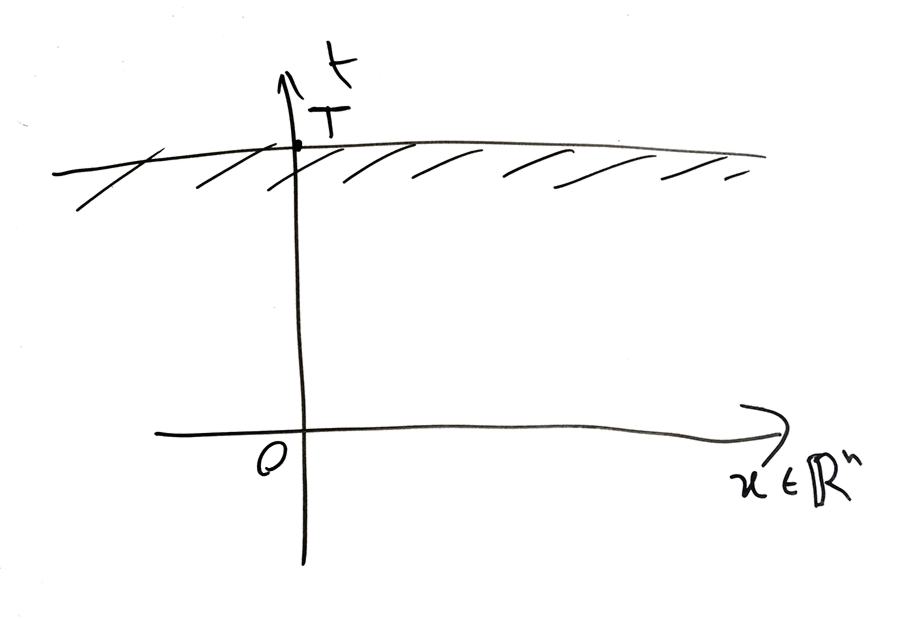
\includegraphics[scale=0.25]{part4.1.png}
\end{center}

Будем рассматривать решения на бесконечных цилиндрах $$u : \real^+ \times \real^n \rightarrow \real,$$ 
ограниченные в каждой ограниченной полосе: 
\begin{equation}
	\forall T > 0 \quad \exists C = C(T) > 0 : \quad |u(t, x)| \leq C(T) \quad \forall t \in [0, T] \quad \forall x \in \real^n.
\label{условие во всем пространстве}
\end{equation}

\begin{theorem}[Принцип максимума для уравнения теплопроводности во всем пространстве]
Пусть поставлена задача Коши для уравнения теплопроводности в $\real^n$ \eqref{heathomcauchy}, и $T > 0$. Тогда для решения, ограниченного в каждой ограниченной полосе верно, что супремум по всей полосе равен супремуму по нижней границе полосы:
$$ M_+ = \sup_{\stackrel{x \in \real^n,} {t \in [0, T]}}u(t,x), \quad N_+ = \sup_{x \in \real^n} u(0, x), \quad M_+ = N_+ $$

\begin{note}
Очевидно, $-\infty < N_+ \leq M_+ < +\infty.$
\end{note}
\end{theorem}

\begin{proof}
Вспомним обозначения для оператора теплопроводности:
$$ Lu = u_t - a^2 \Delta u.$$
Пусть $\eps >0 $ и $u$ --- решение уравнения теплопроводности во всем пространстве. Рассмотрим
$$v_\eps(t, x) = u(t, x) - \eps(2na^2t + \abs{x}^2).$$
Тогда
$$Lv_\eps = Lu - \eps L(2na^2t + \abs{x}^2) = -\eps(2na^2 - a^2\Delta\abs{x}^2) = -\eps(2na^2 - 2na^2) = 0.$$
Таким образом, $v_\eps$ --- тоже решение уравнения теплопроводности во всем пространстве.

Рассмотрим открытые цилиндры: $$Q_{T,R} = (0,T)\times B_R(0).$$

\begin{center}
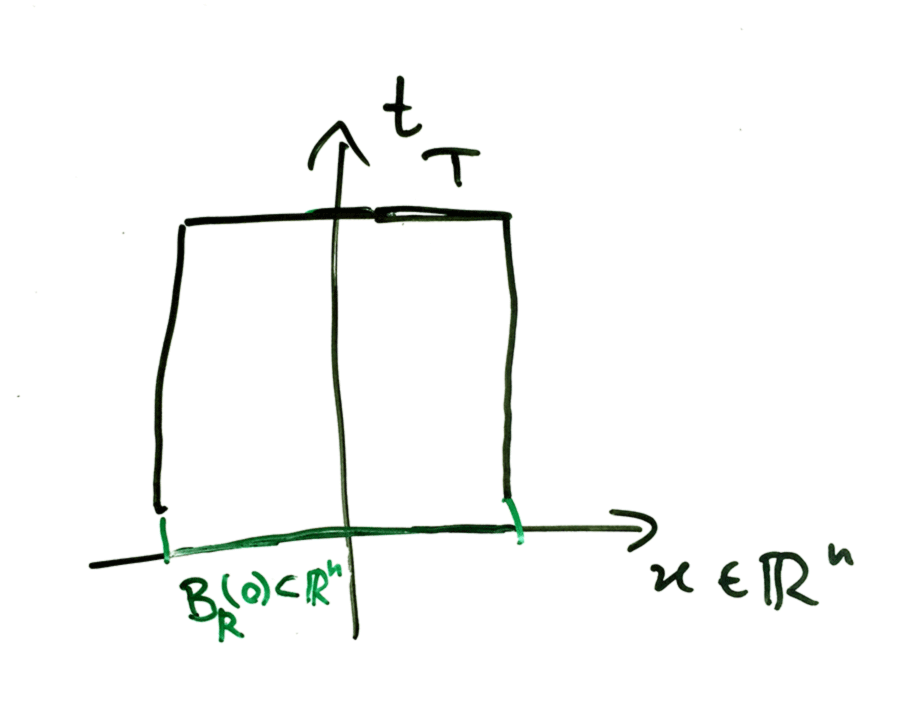
\includegraphics[scale=0.25]{part4.2.png}
\end{center}

Можно заметить, что полоса равна объединению всех таких цилиндров по $R$. По принципу максимума в ограниченной области максимум и минимум достигаются на параболической границе. На нижней крышке имеем
$$ v_\eps (0,x) = u(0,x) - \eps |x|^2 \leq N_+ \quad$$
На боковой поверхности:
$$v_\eps(t,x)\Bigg\rvert_{\abs{x} = R} = u(t,x) \Bigg\rvert_{\abs{x} = R} - \eps(2na^2t + R^2) \leq u(t,x)\Bigg\rvert_{\abs{x} = R} - \eps R^2 \leq M_+ - \eps R^2$$
Для любого $\eps$ можно подобрать такой $R_\eps$, чтобы было верно неравенство $$ M_+ - \eps R^2_\eps \leq N_+.$$

Таким образом,
$$ v_\eps (t, x) \leq N_+ \quad \forall (t,x) \in {Q_{T, R_\eps}}$$
Осталось доказать, что
$$u(t,x) \leq N_+, \quad \forall (t,x) \in [0, T] \times \real^n$$
Фиксируем произвольную точку $(t,x)$. Начиная с какого-то $\eps_0$ она будет лежать в цилиндрах $Q_{T, R_\eps}$, и станет верно
$$v_\eps(t,x) = u(t,x) - \eps(2na^2t - \abs{x}^2) \leq N_+ \quad \forall \eps \geq \eps_0$$
То есть,
$$u(t,x) \leq N_+ + \eps \underbrace{(2na^2t + |x|^2)}_{const}$$
Устремив $\eps$ к нулю, получаем искомое соотношение.

\end{proof}

\begin{corollary}[Принцип минимума для уравнения теплопроводности во всем пространстве]
$$M_- = \inf_{\stackrel{x \in \real^n, \,} {t \in [0, T]}}u(t,x); \qquad N_- = \inf_{x \in \real^n}u(0,x),$$
то $M_-=N_-$ (инфимум по полосе равен инфимуму по нижней границе).
\end{corollary}

\begin{corollary}[Единственность]
Рассмотрим задачу Коши для неоднородного уравнения:
\begin{align}
    \begin{cases} 
        u_t - a^2 \Delta u = q, \\
        u (0, x) = \varphi (x).
    \end{cases}
\label{heatnonhomcauchy}
\end{align}
Классическое решение для задачи \eqref{heatnonhomcauchy} --- единственное в классе функций, ограниченных в каждой полосе.
\end{corollary}

\begin{proof}
Пусть $u_1, \, u_2 $ --- два решения. $L$ --- оператор теплопроводности.  Тогда
\begin{align*}
	\begin{cases*}
		Lu_1 = Lu_2 = q, \\
		u_1\Big\rvert_{t=0} = u_2\Big\rvert_{t=0} = \varphi(x),
	\end{cases*}
	\quad \Rightarrow \quad
	\begin{cases*}
		L(u_1 - u_2) = 0, \\
		\quad (u_1-u_2) \Big\rvert_{t=0}=0.
	\end{cases*}
\end{align*}

Таким образом, $u = u_1 - u_2$ --- решение однородной задачи с нулевыми начальными условиями (в том же классе ограниченных в полосе функций). Значит, по доказанной теореме супремум и инфимум $u$ равны нулю, и, следовательно, $u1 = u2$.

\end{proof}

\begin{note}
Условие ограниченности в каждой полосе необходимо, так как без него решение не будет единственным: кроме решения в полосе будет еще и некое быстрорастущее решение. Неединственность относится уже не к теплопроводности, поэтому физики тоже накладывают ограничения, чтобы получать единственное решение.
\end{note}


\subsection{Фундаментальное решение уравнения теплопроводности}
Пусть стоит задача Коши для однородного уравнения теплопроводности в $\real^n$:
\begin{align*}
	\begin{cases*}
		u_t - a^2 \Delta u = 0, \\
		u(0,x) = \varphi(x).
	\end{cases*}
\end{align*}

Пока что забудем про начальное условие.

\begin{definition} Общее решение уравнения
$$ u_t - a^2 \Delta u = 0$$
называется фундаментательным решением уравнения теплопроводности.
\end{definition}

Заметим, что производная по $t$ первого порядка, а по $x$ --- второго. Значит, решение такого уравнения "хорошо" себя ведёт при растяжении времени и координат: например, если растянуть время в $\lambda$ раз, а пространство в $\lambda^2$ раз, то решение не изменится.

Не умаляя общности, можно считать, что $a = 1$.

\begin{enumerate}
\item Ищем решение, инвариантное относительно растяжений:
$$u(t,x) = \lambda^\alpha u(\lambda t, \lambda^\beta x) \quad \forall \lambda$$

Пусть $\lambda = \dfrac{1} {t}$ и $u(1, z) = v(z)$. Тогда
$$u(t,x) = \frac{1}{t^\alpha} u \left( 1, \frac{x}{t^\beta} \right) = \frac {1} {t^\alpha} v \left( \frac{x}{t^\beta} \right).$$

Посчитаем $Lu$. Так как
$$\frac{\partial}{\partial t} \left(v\left( \frac{x}{t^\beta}\right)\right) = \sum \limits_{i=1}^n \frac{ \partial v}{\partial x_i}\left(\frac{x}{t^\beta}\right) \cdot \frac{-\beta x_i}{t^{\beta + 1}} = -\frac{\beta}{t^{\beta + 1}}\nabla v\left( \frac{x}{t^\beta}\right) \cdot x,$$
то
$$Lu = -\frac{\alpha}{t^{\alpha + 1}} v\left( \dfrac{x}{t^\beta}\right) - \dfrac{\beta}{t^{\alpha + \beta + 1}}\nabla v\left( \dfrac{x}{t^\beta}\right)\cdot x - \dfrac{1}{t^\alpha t^{2\beta}}\Delta v\left( \dfrac{x}{t^\beta}\right) = 0.$$

Сделаем замену $ y = \dfrac{x} {t^\beta}$:
$$Lu =  \dfrac{\alpha}{t^{\alpha + 1}} v(y) + \dfrac{\beta}{t^{\alpha + 1}} \nabla v(y) \cdot y + \dfrac{1}{t^\alpha  t^{2\beta}}\Delta v(y)=0.$$

Положим $\beta = \dfrac{1}{2}$ и умножим полученное выражение на $t^{\alpha + 1}:$
$$\alpha v(y) + \dfrac{1}{2} \nabla v(y) \cdot y + \Delta v(y) = 0.$$

\item Ищем радиальное решение:
$$u(t,x) = \tilde{u}(t,|x|), \quad v(y) = w(|y|).$$
Пусть $r = |y|$. Пересчитаем лапласиан:
\begin{gather*}
	\quad \Delta v(y) = \dfrac{\partial^2v}{\partial y_1^2} + \dots + \dfrac{\partial^2v}{\partial y_n^2}, \\
	\begin{cases*}
		\dfrac{\partial w}{\partial y_i} = w' \dfrac{\partial |y|}{\partial y_i} = w' \dfrac{y_i}{r}, \\
		\dfrac{\partial^2 w}{\partial y_i^2} = w''\dfrac{y_i^2}{r^2} + w'\left(\dfrac{1}{r} - \dfrac{y_i^2}{r^2}\right),
	\end{cases*}
	\quad \Rightarrow \quad
	\Delta w(r) = \dfrac{w''}{r^2}\sum \limits_{i=1}^n y_i^2 + \dfrac{w'}{r}\sum \limits_{i=1}^n (1 - \dfrac{y_i^2}{r^2}) = w'' + \dfrac{w'n}{r},
\end{gather*}
Перепишем результат предыдущего пункта:
$$ \alpha w(r) + \dfrac{1}{2} w'(r) \cdot r + w''(r) + \dfrac{n-1}{r}w'(r) = 0.$$
Положим $\alpha = \dfrac{n}{2}$. Заметим, что здесь стоит сумма двух производных:
$$ \dfrac{n}{2}w(r) + \dfrac{1}{2}w'(r) \cdot r + w''(r) + \dfrac{n-1}{r}w'(r) = \dfrac{1}{2}\left(r^nw\right)' + \left(r^{n-1}w'\right)' = 0.$$
Значит,
$$ \dfrac{1}{2} r^n w+ r^{n-1} w' = \gamma. $$

\item По физическим соображениям наше решение должно быстро убывать на бесконечности:
$$ \lim_{r \to \infty} r^a w' + r^b w = 0 \quad \forall a ,b \in \real$$
Это возможно только тогда, когда $\gamma = 0$. Осталось решить уравнение
$$w' + \frac {r} {2} w = 0.$$
Считаем:
$$ \frac {dw} {w} = - \frac {r} {2} \, dr \quad \Rightarrow \quad w(r) = b e^ {- \frac {r^2} {4}}.$$
Нашли решение, инвариантное относительно растяжений, радиальное и убывающее на бесконечности быстрее любого полинома.

Подставив, получаем однопараметрическое семейство решений:
$$ u(t,x) = \frac {1} {\sqrt{t^n}} w \left( \frac {|x|} {\sqrt{t}} \right) = \frac {b} {\sqrt{t^n}} e^{-\frac {|x|^2} {4t} }, \quad b > 0 $$

\item Осталось выбрать константу $b$. Отнормируем:
$$ \int \limits_{\real^n} u(t,x) \, dx = 1.$$
\begin{exercise} Вычислить $b$.
\end{exercise}
Правильный ответ: $b = \dfrac {1} {\sqrt{(4\pi)^n}}$
\end{enumerate}

\begin{definition}
Фундаментальным решением уравнения теплопроводности называется функция
$$ \Phi(t, x) = \frac {1} {\sqrt{(4 \pi t)^n}} e ^ {- \frac {|x|^2} {4t}}.$$
\end{definition}

\begin{exercise}
Что получится, если $a \not= 1$?
\end{exercise}

\begin{note}
При фиксированном $t$ полученное выражение --- гауссова функция (плотность нормального распределения):

\begin{center}
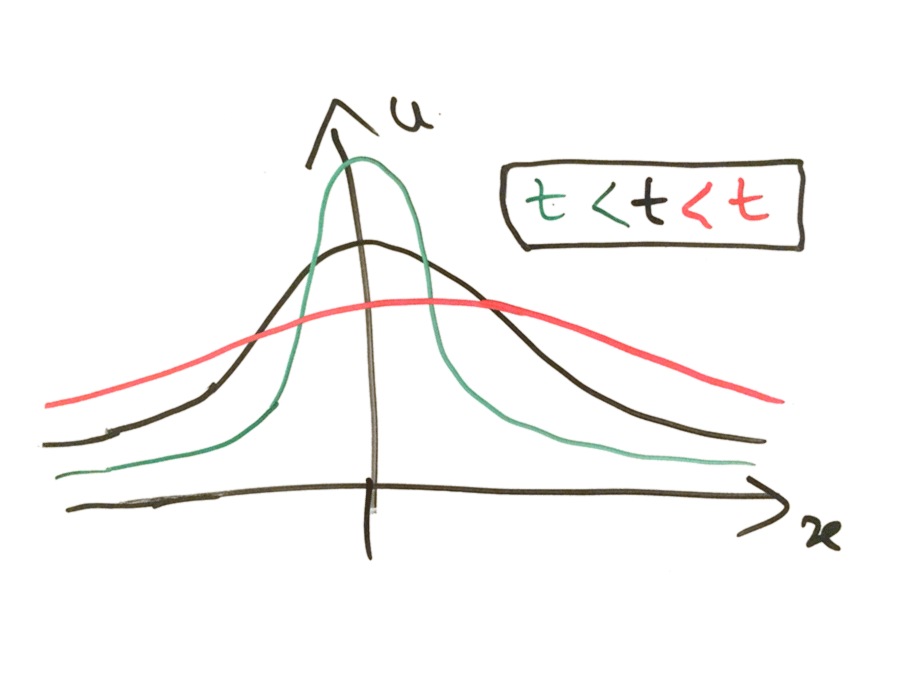
\includegraphics[scale=0.3]{part4.3.png}
\end{center}

Чем меньше $t$, тем выше пик на графике. При $t \to 0$ гауссиана стремится равномерно к нулю везде кроме точки $0$. В точке $0$ она уходит в бесконечность.
\end{note}

\begin{theorem}[Интегральная формула для решения задачи Коши]
Пусть $\varphi\in C_b(\real^n)$ --- ограниченная и непрерывная (начальное распределение), а $u$ задаётся формулой
$$u(t,x) = (\Phi(t) * \varphi) (x) =  \int\limits_{\real^n}\Phi(t, x-y)\varphi(y) \, dy.$$
Тогда $u$
\begin{enumerate}
\item бесконечно гладкая: $$u \in C^\infty\left(\left(0, +\infty\right)\times \real^n\right)$$
\item удовлетворяет уравнению теплопроводности: $$ u_t - \Delta u = 0$$
\item удовлетворяет начальному условию: $$\lim\limits_{(t,\,y) \rightarrow (0,\,x)}u(t,x) = \varphi (x).$$
\end{enumerate}

Иначе говоря, для получения решения задачи Коши для уравнения теплопроводности с ограниченным начальным условием достаточно свернуть начальное условие с фундаментальным решением.
\end{theorem}

\begin{proof}
\begin{enumerate} 
\item Очевидно, $\Phi \in  C^\infty\left(\left(0, +\infty\right)\times \real^n\right)$. Производные проносятся под интеграл:
$$u_t = \int\limits_{\real^n} \Phi_t(t,x-y)\varphi(y) \, dy, \quad u_{x_i} = \int\limits_{\real^n} \Phi_{x_i}(t, x-y)\varphi(y) \, dy$$
Значит, $u \in C^\infty.$
\item Применим оператор теплопроводности: $$Lu = u_t - \Delta u = \int\limits_{\real^n} \underbrace{(\Phi_t - \Delta \Phi)(t, x-y)}_{0}\varphi(y) \, dy = 0.$$
\item Пусть $x_0 \in \real^n$. Посчитаем предел по определению. Для начала,
\begin{align*}
|u(t,x) - \varphi(x_0)| &= \Bigl| \int \limits_{\real^n} \Phi(t, x-y) \varphi(y) \, dy - \varphi(x_0) \Bigl| = \\
	&= \Bigl| \int \limits_{\real^n} \Phi(t, x-y) \varphi(y) \, dy - \varphi(x_0) \int \limits_{\real^n} \Phi(t, x-y) \, dy\Bigl|= \\
	&= \Bigl| \int \limits_{\real^n} \Phi(t, x-y) (\varphi(y) - \varphi(x_0)) \, dy \Bigl| \leq \int \limits_{\real^n} \Phi(t, x-y) \, \bigl| \varphi(y) - \varphi(x_0) \bigl| \, dy = \\
	&= \underbrace {\int \limits_{B_\delta (x_0)} \Phi(t, x-y) \, \bigl| \varphi(y) - \varphi(x_0) \bigl| \, dy}_{I_\delta} + \underbrace {\int \limits_{B^c_\delta (x_0)} \Phi(t, x-y) \, \bigl| \varphi(y) - \varphi(x_0) \bigl| \, dy}_{J_\delta}.
\end{align*}
Мы внесли $\varphi(x_0)$ под знак интеграла, оценили его сверху и разбили оценку на два интеграла: по $\delta$-окрестности $x_0$ и по её дополнению.

Пусть $\eps > 0$. Функция $\varphi$ непрерывна. Значит, можно выбрать такое $\delta$, что 
$$ | \varphi(y) - \varphi(x_0)| < \dfrac {\eps} {2} \quad \forall y \in B_\delta (x_0)$$

Тогда
$$ I_\delta \leq \int \limits_{\real^n} \Phi(t, x-y) \, \frac {\eps} {2} \, dy = \frac {\eps} {2}. $$

Пусть $|x - x_0| < \dfrac{\delta}{2}$, тогда при $y \notin B_\delta(x_0)$ верно $|x - y| \geq \dfrac{1}{2}|x_0 - y|.$
Оцениваем $J_\delta$:
\begin{align*}
J_\delta & \leq 2 || \varphi ||_\infty \int \limits_{B^c_\delta (x_0)} \Phi(t, x-y) \, dy = 2 || \varphi ||_\infty \frac {1} {\sqrt{(4 \pi t)^n}} \int \limits_{B^c_\delta (x_0)} e^{- \frac {|x - y|^2} {4t}} \, dy \leq \\
 & \leq 2 || \varphi ||_\infty \frac {1} {\sqrt{(4 \pi t)^n}} \int \limits_{B^c_\delta (x_0)} e^{- \frac {|x_0 - y|^2} {16t}} \, dy \leq \frac {C} {\sqrt{(4 \pi t)^n}} \int \limits_\delta^{+\infty} e^{- \frac {\rho^2} {16t}} \rho^{n-1} \, d\rho = \\
 &= C \int \limits_{\delta / \sqrt{t}}^{+\infty} e^{- \frac {r^2} {16t}} r^{n-1} \, dr \stackrel{t \to 0} {\longrightarrow} 0
\end{align*}
Мы оценили модуль под знаком суммой модулей, а сумму оценили удвоенной равномерной нормой. Далее мы воспользовались неравенством, перешли к сферическим координатам и сделали замену $r = \dfrac {\rho} {\sqrt{t}}$. 

Можем выбрать такое $t$, что $$ t \leq \frac {\delta} {2}, \quad J_\delta \leq \dfrac {\eps} {2}.$$
Суммируем $I_\delta$ и $J_\delta$. Тогда
$$ \forall \eps >0 \quad \exists t, \delta: \quad | x- x_0| < \frac {\delta} {2} \quad \& \quad |t| < \frac {\delta} {2} \quad \Rightarrow \quad |u(t,x) - \varphi(x_0)| < \eps,$$
что и требовалось доказать.
\end{enumerate}

\end{proof}


\subsection{Решение задачи Коши для неоднородного уравнения теплопроводности в пространстве. Метод Дюамеля}
Поставим начальную задачу для неоднородного уравнения теплопроводности в $\real^n$:
\begin{align}
    \begin{cases} 
        u_t - \Delta u = f(t,x), \\
        u (0, x) = \varphi (x).
    \end{cases}
\label{heatnonhomcauchy2}
\end{align}


\begin{note}[Принцип суперпозиции]
Пусть $u_1$, $u_2$ --- решения задач
\begin{equation*}
\begin{cases} 
        Lu_1 = f, \\
        u_1\Bigl|_{t=0} = 0,
    \end{cases}
    \quad \text{и} \quad
    \begin{cases} 
        Lu_2 = 0, \\
        u_2\Bigl|_{t=0} = \varphi (x),
    \end{cases}
\end{equation*}
соответственно. Тогда $u = u_1+u_2$ --- решение задачи \eqref{heatnonhomcauchy2}
\end{note}

Не умаляя общности, считаем, что $\varphi = 0$.

\subsubsection*{Принцип Дюамеля}

Пусть $v(t,x,s)$ --- решение семейства задач
\begin{equation*}
    \begin{cases} 
        v_t - \Delta v = 0, \\
        v\Bigl|_{t=s} = f(s, .).
    \end{cases}
\end{equation*}

$$u(t,x) = \int\limits_0^tv(t,x,s) \, ds = \int\limits_0^t \, ds \int\limits_{\real^n}\Phi(t-s, x-y)f(s,y) \, dy.$$

В некоторых случаях эта формула даёт классическое решение, рассмотрим один из них:

\begin{theorem}
Пусть $$u(t,x) = \int\limits_0^t ds \int \limits_{\real^n} \Phi (t-s, x-y) f(s,y) \, dy ,$$ и функция $f\in C_x^2 \cap C_t^1$, а также финитная в $(0, \infty) \times \real^n$. Тогда $u$
\begin{enumerate}
\item непрерывно дифференцируема один раз по $t$ и два раза по $x$: $$u \in C_t^1 \cap C_x^2,$$
\item является решением задачи Коши для неоднородного уравнения теплопроводности: $$u_t - \Delta u = f, \quad u(0,x) = 0,$$
\item удовлетворяет начальному условию: $$\lim_{(t,x) \to (0,x_0)} u(t,x) = 0 \quad  \forall x_0 \in \real^n.$$
\end{enumerate}
\end{theorem}

\begin{proof}

\begin{enumerate}
\item Взять и пронести производную под знак интеграла не можем, так как в точке $t = s$ у $\Phi$ имеется сингулярность. Поменяем переменные в свёртке:
$$ u(t, x) = \int \limits_0^t ds \int \limits_{\real^n} \Phi(s,y) f(t-s, x-y) \,dy.$$
Теперь можем проносить производные по $x$:
$$ \Delta u = \int \limits_0^t ds \int \limits_{\real^n} \Phi(s,y) \Delta f (t-s, x-y) \, dy.$$
Со временем немного сложнее из-за переменного верхнего предела:
$$  u_t = \int \limits_{\real^n} \Phi(t,y) f(0, x-y) \, dy + \int \limits_0^t ds \int \limits_{\real^n} \Phi(s,y) f_t(t-s,x-y) \, dy.$$
\item Подставляем в уравнение:
$$ u_t - \Delta u = \int \limits_{\real^n} \Phi(t,y) f(0, x-y) \, dy +  \int \limits_0^t ds \int \limits_{\real^n} \Phi(s,y) \left( \pder{t} - \Delta_x \right) f(t-s, x-y) \, dy.$$
% цитирую: "Было бы неплохо "перекинуть" дифференциальный оператор с $f$ на $\Phi$."
Заметим, что
$$ \pder{t} f(t-s,x-y) = - \pder{s} f(t-s, x-y), \quad \Delta_x f(t-s, x-y) = \Delta_y f(t-s, x-y)$$
Тогда
$$ u_t - \Delta u = \int \limits_{\real^n} \Phi(t,y) f(0, x-y) \, dy +  \int \limits_0^t ds \int \limits_{\real^n} \Phi(s,y) \left( -\pder{s} - \Delta_y \right) f(t-s, x-y) \, dy.$$
Пусть $\eps > 0$. Разобъём второй интеграл на два:
\begin{gather*}
\int \limits_0^t ds \int \limits_{\real^n} \Phi(s,y) (-\pder{s} - \Delta_y) f(t-s, x-y) \, dy = I_1 + I_2 = \\ 
= \int \limits_0^\eps ds \int \limits_{\real^n} \Phi(s,y) \left(-\pder{s} - \Delta_y \right) f(t-s, x-y) \, dy \\
+ \int \limits_\eps^t ds \int \limits_{\real^n} \Phi(s,y) \left( -\pder{s} - \Delta_y \right) f(t-s, x-y) \, dy.
\end{gather*}
В $I_1$ производные $f$ финитны, можно оценить их равномерными нормами и вынести за знак интеграла:
$$I_1 \leq (|| f_t ||_\infty + || \Delta f ||_\infty) \int \limits_0^\eps ds \underbrace {\int \limits_{\real^n} \Phi(s,y) \, dy }_{=1} = C \eps \stackrel {\eps \to 0} {\longrightarrow} 0. $$
В $I_2$ интегрированием по частям можно перенести дифференциальный оператор на $\Phi$, в этом нам поможет финитность $f$:
\begin{align*}
	I_2 &= \int \limits_\eps^t ds \int \limits_{\real^n} \Phi(s,y) \left( - \pder{s} - \Delta_y \right) f(t-s, x-y) \, dy = \\
	&= \int \limits_\eps^t ds \int \limits_{\real^n} (\underbrace {\Phi_s - \Delta_y\Phi}_{=0})(s,y) f(t-s, x-y) \, dy \\
	& +  \int \limits_{\real^n} \Phi(\eps, y) f(t - \eps, x-y) \, dy - \int \limits_{\real^n} \Phi(t, y) f(0, x-y) \, dy.
\end{align*} 
Интегрировали мы по $(\eps, t) \times K$, где $K$ --- некоторый компакт. На боковых границах функция $f$ равна нулю, так что граничные члены остались только с верхней и нижней "крышек".

Таким образом, для всех $(t,x)$ верно
$$ u_t - \Delta u = \lim_{\eps \to 0} \int \limits_{\real^n} \Phi(\eps, y) f(t-\eps, x-y) \, dy = f(t,x).$$

\item Оценим по модулю, попутно воспользовавшись финитностью:
$$\abs{u(t,x)} \leq \int \limits_0^t ds \int \limits_{\real^n} \Phi(s,y) |f(t-s, x-y)| \,dy \leq C \int \limits_0^t ds \int \limits_{\real^n} \Phi(s,y) \, dy = Ct \stackrel{t \to 0} \longrightarrow 0. $$
\end{enumerate}

\end{proof}

\subsection{Уравнения Лапласа и Пуассона}
\begin{definition}
Пусть $\Omega \subset \real^n$ - область, $x \in \Omega$. Тогда уравнения
\begin{equation}
    - \Delta u(x) = 0,
\label{Laplace}
\end{equation}
\begin{equation}
    -\Delta u(x) = f(x)
\label{Poisson}
\end{equation}
называются уравнением Лапласа и уравнением Пуассона соответственно. 
\end{definition}

Эти уравнения описывают стационарное температурное поле в области $\Omega$, в которой плотность источников и стоков теплоты не зависит от времени.

Есть ещё и электростатическая интерпретация. В таком случае уравнение Пуассона описывает распределение потенциала электростатического поля $u$ с плотностью заряда $f$.

Обычно для уравнений Лапласа и Пуассона ставится одна из двух задач:

\subsubsection{Задача Дирихле}
$$u \Bigg \rvert_{\partial\Omega} = u_0.$$
Это условие означает, что задана температура или потенциал на границе области. 

\subsubsection{Задача Неймана}
$$\dfrac{\partial u}{\partial n}\Bigg\rvert_{\partial\Omega} = 0.$$
Это условие означает идеально изолированную область.